\subsubsection{ソフトウェア設計原則}

設計原則は、設計中の判断に方向を与える基本的な考え方である。原則は、特定のプログラミング言語や開発手法だけに依存しない。むしろ、複雑な問題を扱うための共通の知恵である。

\par\smallskip\noindent\refstepcounter{table}\label{tab:ch03-03}\textbf{表 \thetable: 第03章 ソフトウェア設計 表03}\par\smallskip
\begin{longtable}{L{34mm}L{55mm}L{76mm}}
\toprule
\textbf{原則} & \textbf{意味} & \textbf{実務で見ること} \\
\midrule
\endhead
抽象化 & 目的に関係する情報だけを示し、不要な詳細を隠す。 & 利用者、設計者、実装者が必要な詳細水準だけを見られるか。 \\
関心事の分離 & 異なる関心を分けて扱う。 & 業務処理、認証、ログ、表示、保存などが混ざりすぎていないか。 \\
モジュール化 & 大きなソフトウェアを小さな部品へ分ける。 & 各部品の責務が明確で、独立して理解・変更できるか。 \\
カプセル化・情報隠蔽 & 内部詳細を隠し、必要なインタフェースだけを見せる。 & 外部が内部データ構造や実装順序に依存していないか。 \\
インタフェースと実装の分離 & 外部に見せる契約と内部実装を分ける。 & 実装を変えても、利用側の変更が少なく済むか。 \\
結合度 & 部品同士の依存の強さである。 & ひとつの部品変更が多数の部品変更を引き起こさないか。 \\
凝集度 & ひとつの部品内の要素がどれだけ関連しているかである。 & ひとつの部品が複数の無関係な責務を抱えていないか。 \\
一貫性 & 名前、記法、順序、インタフェースなどをそろえる。 & 似た問題に似た解決策を使っているか。 \\
完全性 & 重要な特徴や要求を漏らさない。 & 通常時、例外時、境界条件、状態、モードが考慮されているか。 \\
検証可能性 & 要求や制約を満たすか確認できる。 & 設計からテスト、レビュー、分析が可能か。 \\
倫理的配慮 & 人権、福祉、透明性、説明責任、悪用可能性などを考慮する。 & AI、自律システム、社会的影響があるシステムで設計上の配慮があるか。 \\
\bottomrule
\end{longtable}

特に、結合度と凝集度は初学者が最初に押さえるべき設計観点である。一般に、よい設計は、部品間の結合度を低くし、部品内の凝集度を高くする。結合度が高いと変更の影響が広がる。凝集度が低いと、部品が何を担当しているのか理解しにくくなる。

\begin{pointbox}{重要}
設計原則は、単独で使うものではない。抽象化、関心事の分離、モジュール化、カプセル化、低結合、高凝集は互いに支え合う。
\end{pointbox}

\begin{figure}[htbp]
\centering
\IfFileExists{assets/fig-ch03-04.png}{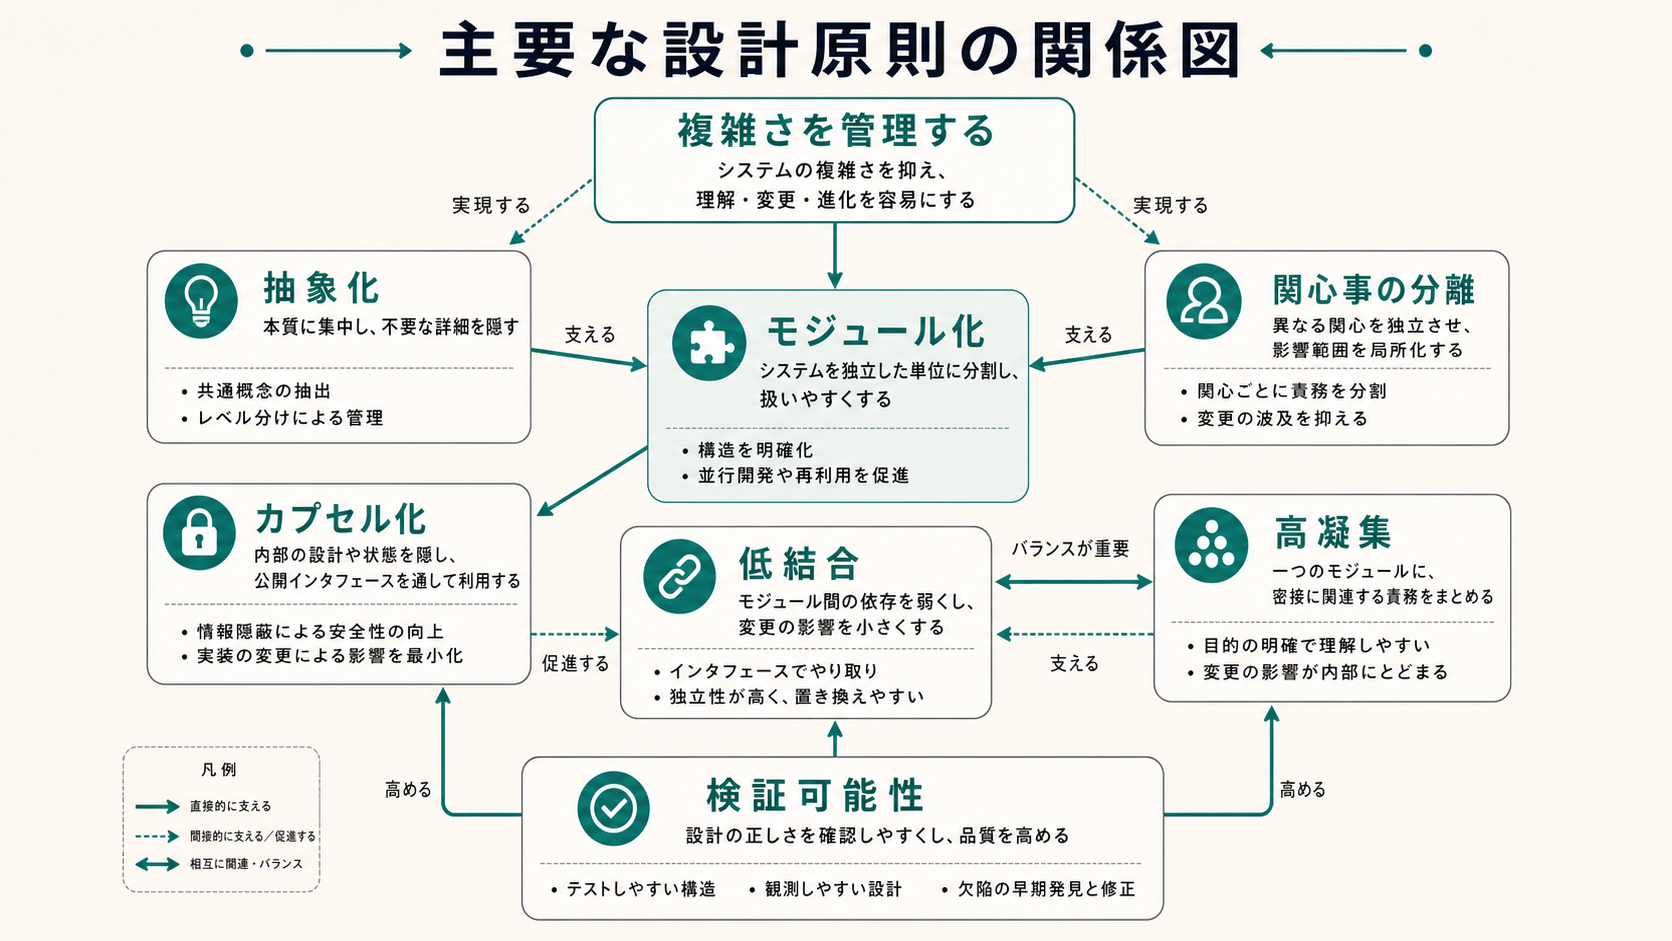
\includegraphics[width=0.96\linewidth]{assets/fig-ch03-04.png}}{\fbox{\parbox[c][48mm][c]{0.9\linewidth}{\centering 画像生成待ち\\主要な設計原則の関係図}}}
\caption{主要な設計原則の関係図}
\label{fig:ch03-04}
\end{figure}
